\section{Introduction}\label{sec:introduction}
Electrical schematics encode engineering decisions through relations among terminals, conductors, contacts, and devices. During drawing inspection or maintenance preparation, an engineer may need to determine whether opening a contact disconnects a branch, identify faults consistent with continuity readings, or assess whether a proposed connection satisfies a stated requirement. These questions depend on the interaction between visible topology and explicitly specified conditions. Correct recognition of component names alone is insufficient: overlooking a short conductor, assuming an unsupported junction, or confusing an unknown contact state with a closed contact can reverse the answer.

Figure~\ref{fig:introcase} illustrates this challenge through a measurement-planning record associated with an original DWG circuit window in \dataset. Given three candidate single-contact faults, the task is to choose the fewest continuity measurements that distinguish their outcomes. The upstream contact is common to the relevant branches, whereas the two downstream contacts affect different branches. Measurements at 1DK6:4 and JD1:1 therefore distinguish an upstream interruption from the two branch-specific faults. The model must combine terminal grounding, wiring topology, and explicit fault assumptions before selecting these informative test points. The compact fault-signature table explains both why two tests suffice and why a single binary measurement cannot suffice. This example motivates annotations that supervise an engineering decision together with a checkable justification, rather than label recognition alone.

\begin{figure*}[t]
\centering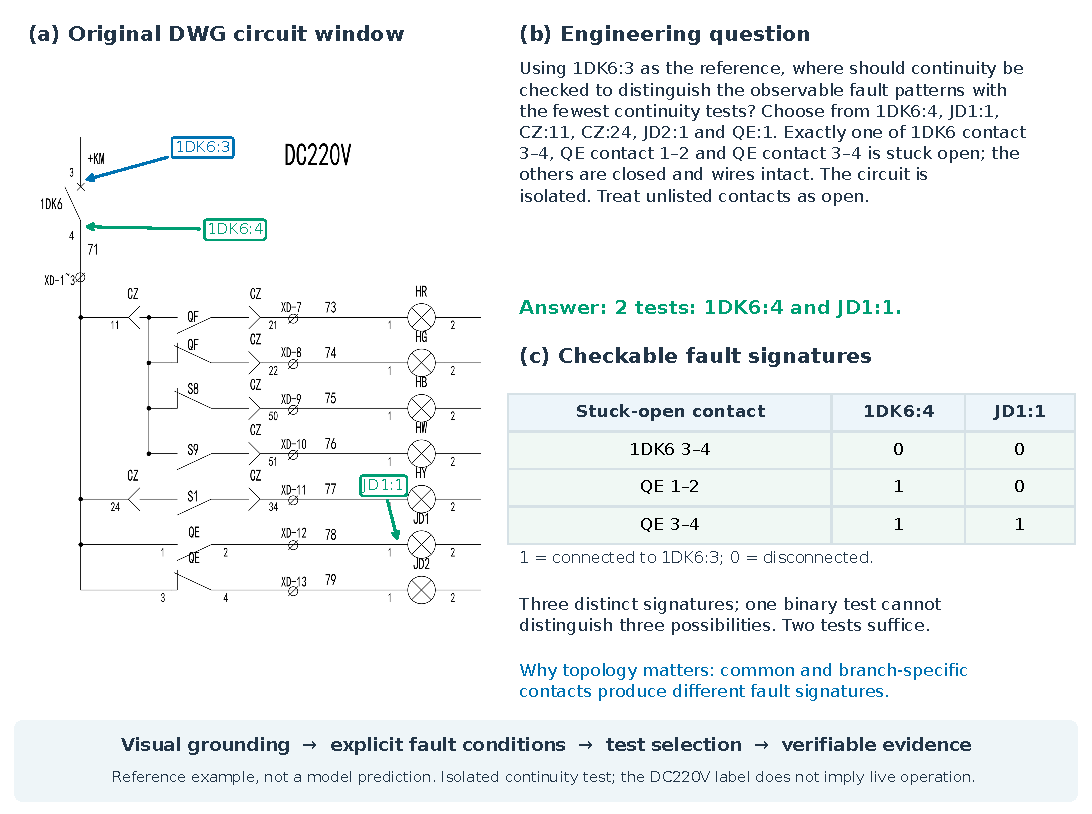
\includegraphics[width=\textwidth]{assets/figure_01.pdf}
\caption{An illustrative \dataset measurement-planning example from the training partition, using an original DWG window. The released question and answer appear beside compact reference evidence. Continuity tests at 1DK6:4 and JD1:1 give distinct signatures $(0,0)$, $(1,0)$, and $(1,1)$ for the three candidate faults; a single binary measurement cannot distinguish all three. Rendering adjustments and editorial callouts preserve the original wiring topology. The associated graph queries verify the stated fault signatures.}
\label{fig:introcase}
\end{figure*}

Visual question answering (VQA) offers a natural-language interface to this information. Document-oriented benchmarks establish the importance of reading text within its visual context~\cite{singh2019textvqa,mathew2021docvqa}, while diagram and chart benchmarks examine relations that cannot be recovered from isolated labels~\cite{kembhavi2016diagram,masry2022chartqa}. Recent engineering benchmarks extend this direction toward professional artifacts. DrawingVQA evaluates construction drawings through perceptual, contextual, and domain-expert questions~\cite{jung2026drawingvqa}; DesignQA examines engineering requirements and documentation~\cite{doris2025designqa}; and MechVQA addresses mechanical drawing interpretation~\cite{kou2026mechvqa}. Together, these studies motivate task definitions grounded in engineering practice rather than generic image description.

Electrical diagram understanding is itself an established research area. CircuitVQA, ElectroVizQA, and EEE-Bench cover circuit images, educational electronics, and broader electrical engineering problems, respectively~\cite{mehta2024circuitvqa,meshram2024electrovizqa,li2025eeebench}. CircuitSense studies visual-to-symbolic circuit analysis~\cite{akbari2025circuitsense}, and OmniSch evaluates schematic grounding and graph construction~\cite{lu2026omnisch}. The complementary question considered here is how to construct reusable training and evaluation data for local engineering decisions in native electrical drawings, with inspectable evidence and reproducible state-dependent labels.

Three requirements follow. First, annotations must connect a natural-language conclusion to identifiable visual and electrical entities. A plausible explanation is insufficient unless its stated route, blocking condition, or diagnostic alternative can be checked. Second, the question must distinguish what is drawn from what is assumed. A static schematic does not establish the present voltage or operating state of equipment. Third, evaluation must account for dependencies among questions, overlapping windows, and edited versions of the same source circuit. Treating these observations as independent can overstate generalization to unseen engineering documents.

We address these requirements through \dataset, a dataset derived from native computer-aided design (CAD) drawings. The dataset comprises 10,201 English QA records over 1,019 image configurations, sourced from 44 DWG files across 14 substation projects. Its 300 original context windows and 719 controlled native-DWG variants support tasks involving conditional connectivity, diagnostic ambiguity, measurement selection, and bounded design checks. A short evidence sequence accompanies each answer, while terminal identifiers, source geometry, and executable graph queries retain the underlying verification record. The graph is used to construct and check annotations; it is not supplied as an input to the image-question model.

The dataset also enables a controlled comparison of supervision strategies. We fine-tune the same seven-billion-parameter vision--language backbone with either short answers alone or compact evidence followed by the same answers. Low-rank adaptation (LoRA)~\cite{hu2021lora} provides a standard implementation of domain adaptation. Evidence-guided chain-of-thought denotes externally checkable intermediate statements; it does not imply access to hidden computation or a separately established teacher-distillation process. The empirical objective is to determine where this supervision is beneficial, neutral, or detrimental, rather than to assume a uniform advantage.

The contributions are threefold:
\begin{enumerate}
\item A CAD-derived electrical schematic dataset with 15 task families, concise English questions and answers, compact evidence, and terminal-level provenance.
\item A construction and verification protocol combining native rendering, controlled wiring interventions, executable checks, and source-disjoint partitions.
\item A comparative study design separating general-model benchmarking, controlled answer/evidence supervision, semantic answer correctness, and evidence validity.
\end{enumerate}
The scope is electrical schematic understanding within substation secondary wiring; broader electrical-domain transfer is an empirical question. Section~\ref{sec:related} situates the resource, Section~\ref{sec:dataset} describes its construction, and Sections~\ref{sec:protocol} and~\ref{sec:experiments} specify the comparison and evaluation.
